\documentclass{sig-alternate}

\usepackage{algorithm,array}
\usepackage{todonotes}
\usepackage[noend]{algpseudocode}
\usepackage[bookmarks=false]{hyperref}

\newcommand{\argmax}{\operatorname*{arg\,max}}
\hyphenation{follows}

\begin{document}

\conferenceinfo{GECCO'13,} {July 6--10, 2013, Amsterdam, The Netherlands.} 
\CopyrightYear{2013} 
\crdata{978-1-4503-1963-8/13/07} 
\clubpenalty=10000 
\widowpenalty = 10000


\title{Rolling Horizon Evolution versus Tree Search for Navigation in Single-Player Real-Time Games}

\numberofauthors{4} 
%\author{
%% 1st. author
%\alignauthor
%Anonymous\\
%% 2nd. author
%\alignauthor
%Anonymous\\
%% 3rd. author
%\alignauthor 
%Anonymous\\
%\and
%% 4th. author
%\alignauthor 
%Anonymous\\
%}

%\numberofauthors{4} 
\author{
% 1st. author
\alignauthor
Diego Perez\\
       \affaddr{University of Essex}\\
       \affaddr{Colchester CO4 3SQ}\\
       \affaddr{United Kingdom}\\
       \email{dperez@essex.ac.uk}
% 2nd. author
\alignauthor
Spyridon Samothrakis\\
       \affaddr{University of Essex}\\
       \affaddr{Colchester CO4 3SQ}\\
       \affaddr{United Kingdom}\\
       \email{ssamot@essex.ac.uk}
% 3rd. author
\alignauthor 
Simon M. Lucas\\
       \affaddr{University of Essex}\\
       \affaddr{Colchester CO4 3SQ}\\
       \affaddr{United Kingdom}\\
       \email{sml@essex.ac.uk}
\and
% 4th. author
\alignauthor 
Philipp Rohlfshagen\\
       \affaddr{University of Essex}\\
       \affaddr{Colchester CO4 3SQ}\\
       \affaddr{United Kingdom}\\
       \email{prohlf@essex.ac.uk}
}


\maketitle
\begin{abstract}
In real-time games, agents have limited time to respond to environmental cues. This requires either a policy defined up-front or, if one has access to a generative model, a very efficient rolling horizon search. In this paper, different search techniques are compared in a simple, yet interesting, real-time game known as the Physical Travelling Salesman Problem (PTSP). We introduce a rolling horizon version of a simple evolutionary algorithm that handles macro-actions and compare it against Monte Carlo Tree Search (MCTS), an approach known to perform well in practice, as well as random search. The experimental setup employs a variety of settings for both the action space of the agent as well as the algorithms used. We show that MCTS is able to handle very fine-grained searches whereas evolution performs better as we move to coarser-grained actions; the choice of algorithm becomes irrelevant if the actions are even more coarse-grained. We conclude that evolutionary algorithms can be a viable and competitive alternative to MCTS. 
\end{abstract}

% A category with the (minimum) three required fields
\category{I.2}{Computing Methodologies}{Artificial Intelligence}[learning]
%A category including the fourth, optional field follows...
%\category{D.2.8}{Software Engineering}{Metrics}[complexity measures, performance measures]

%\terms{Algorithms}

\keywords{ai, games, real time, evolutionary algorithms, mcts}

\section{Introduction}

Traditionally, research in Game AI has focused on 2-player perfect information games where the time allowed to make a move is measured in seconds or minutes. Lately, research has started to focus on more complex domains such as those where the whole state of the game is unobserved by the players (as in many card games) or is affected by random events (e.g. in stochastic games like Backgammon). Likewise, real-time constraints have attracted increasing attention, with particular emphasis on video games, where moves need to be made every number of milliseconds. In this paper we will concentrate on the real-time aspect of a game, which requires a search algorithm to converge very fast without much overhead. It is therefore worthwhile to investigate how search methods are able to explore the search space of those games characterised by limited decision time.

The benchmark (and the experimental testbed) used in this paper is the Physical Travelling Salesman Problem (or PTSP), a deterministic single player game that consists of a collection of several waypoints scattered around a map full of obstacles. The challenges here include finding the best sequence of waypoints, as well as the challenge of navigating the player to visit each waypoint in sequence in as little time as possible. This paper focuses in the navigation aspect of the problem. As a real-time game, PTSP provides a small time budget to decide the next move of the player. Additionally, the game allows the player to run simulations in order to foresee the outcome of applying any of the available actions. However, the final state of the game is usually never reached, as the number of moves required to do so by far exceeds the time available to execute them.

As a single-player game, the PTSP allows players that have a model of the game to predict the rewards of the actions taken without any ambiguity. This feature allows the controllers to create precise macro-actions (or repetitions of the same single actions) to reach further states when evaluating the next move to make.

The PTSP has been selected because it holds certain similarities with some modern video-games, at a simplified level. For instance, real-time games need an action to be supplied within a few milliseconds, providing a very limited budget to plan the next move. Furthermore, as in the PTSP, the duration of the game is long enough so the agent is not able to foresee all the outcomes from the moves made. Finally, the fact that the PTSP has featured in international conferences as a competition (see Section~\ref{sec:ptsp}) allows for a direct comparison between the approaches shown here and the ones from the contest.

Four different algorithms are presented in this paper: two versions of a Rolling Horizon Genetic Algorithm (GA and GAC), Rolling Horizon Random Search (RS) and Monte Carlo Tree Search (MCTS). Each one of these algorithms follows a similar scheme in order to solve the problem: first, the order of waypoints to visit is obtained by a common TSP solver. Then, a macro-action handler performs the desired moves while it requests future actions from the appropriate algorithm. Each algorithm performs the search differently, but uses the same value function that evaluates a given state of the game. Therefore, the focus of this paper is on the ability of the algorithm to explore the search space, using different macro-action lengths.

This paper is organised as follows. Section~\ref{sec:lit} discusses tree search and evolutionary algorithms in real-time games. Section~\ref{sec:ptsp} describes the PTSP and Section~\ref{sec:solve} introduces the algorithms and controllers used to play the game. Section~\ref{sec:exp} details the experimental setup and discusses the results obtained. The paper is concluded in Section~\ref{sec:conc}, where some possible extensions of this work are discussed.

\section{Literature review} \label{sec:lit}

\subsection{Monte Carlo Tree Search}

MCTS is a tree search technique that has been widely used in board games, particularly in the game of Go. Go is a territorial board game played in a $19 \times 19$ square grid, in which the two players aim to surround their opponent's stones. The game of Go is considered the drosophila of Game AI, and MCTS players have achieved professional level play in the reduced version of the game ($9\times9$ board size)~\cite{Lee2009}.

MCTS is considered to be \textit{anytime}: the algorithm is able to provide a valid solution (next move in the game) at any moment in time, independently from the number of iterations that have been performed (although more iterations generally produce better results). In contrast, other algorithms (such A*) usually require to have finished to provide an initial action to execute. For this reason, MCTS is a suitable method for real-time domains, and it has been employed extensively in the literature.

A popular real-time game that has been employed as a benchmark for using MCTS is Ms. Pac Man. In this game, the user controls the Pac Man agent with the objective of clearing the maze and eating all the pills without being captured by the ghosts. This game, similar to the PTSP, is open ended (i.e. the end game state is usually not reached within the simulations). Robles et al~\cite{Robles2009} include hand-coded heuristics to guide the simulations towards more promising portions of the search space. Other authors also include domain knowledge from the game to bias the search in MCTS, such as~\cite{Samothrakis, Ikehata2010}.

Regarding single player games, MCTS has been used in several puzzles. Examples are SameGame~\cite{Matsumoto2010}, where the player aims to destroy contiguous items of the same colour distributed in a rectangular grid, or Morpion Solitaire~\cite{Edelkamp2010}, a connection puzzle where the objective is to join vertices of a graph with lines that contain at least five nodes. PTSP itself has been addressed with MCTS techniques, as Perez et al.~\cite{Perez2012b} did to show the importance of adding heuristics to the Monte Carlo (MC) simulations in real-time domains, or Powley et al.~\cite{Powley2012}, who describe the MCTS algorithm that won them the first edition of the PTSP competition.

An extensive survey of Monte Carlo Tree Search methods has been written by Browne et al.~\cite{Browne2012}, where the algorithm, variations and applications are described. It is worth noting that Monte Carlo Tree Search, when combined with UCB1 (see later in this paper) reaches asymptotically logarithmic regret~\cite{coquelin2007bandit}. One can intuitively think of regret as ``opportunity loss''.

%It is worthwhile mentioning that in most cases found in the literature, MCTS techniques have been used with some kind of heuristic that guides the Monte Carlo simulations or the tree selection policy. In the case described in this paper, the simulations are purely random, as the objective is to compare the search abilities of the different algorithms. The intention is therefore to keep the heuristics to a minimum, and the existing pieces of domain knowledge are shared by all the algorithms presented (as in the case of the score function, described later).

\vspace{1cm}
\subsection{Rolling Horizon Evolutionary Algorithms}

When it comes to planning (or control), evolutionary algorithms are mostly used as follows: an evolutionary algorithm is used in conjunction with an off-line simulator in order to train a controller, for example as in~\cite{gomez1999solving}. The controller is then used in the real problem. This approach is not just used for control problems, but has been popular in fields such as Artificial Life (e.g.~\cite{beer1992evolving}). This paper proposes a different approach. Evolution is used in the same manner as MCTS uses roll-outs and the generative model (i.e. a simulator). Thus, an agent will evolve a plan in an imaginary model for some milliseconds, acts on the (real) world by performing the first action of its plan and then evolves a new plan repeatedly (again in a simulation based manner) until the game is over. This type of behaviour is called ``Rolling Horizon'', ``Receding Horizon'' or ``Model Predictive'' control or planning.  There have been some efforts in the past to use such approaches (e.g. \cite{samothrakis2010planning,mercieca2011particle}, and this paper presents two versions of a genetic algorithm in this setting. The term Rolling Horizon comes from the fact that planning happens until a limited look-ahead in the game (and thus we have to keep on replanning at every time step). Contrary to MCTS, we are currently unsure about the regret bounds of genetic algorithms in the general case~\cite{reeves2002genetic}.

\section{The Physical Travelling \\Salesman Problem} \label{sec:ptsp}

The Physical Travelling Salesman Problem (PTSP) is a modification of the well known optimisation problem Travelling Salesman Problem (or TSP).\footnote{TSP consists of an agent who must visit all $n$ cities once via the shortest possible route, starting and ending at the same location.} In the PTSP, the player controls a ship (or agent) that must visit a series of waypoints scattered around a continuous 2-D maze full of obstacles. The score of the game is determined by the number of waypoints visited and the time taken to do so. Figure~\ref{fig:map} shows one of the maps of this game.

%NOTE: Leave this at 0.35. If it is to be made clearer, generate the image again with larger text font.
\begin{figure} [!t]
	\begin{center}
	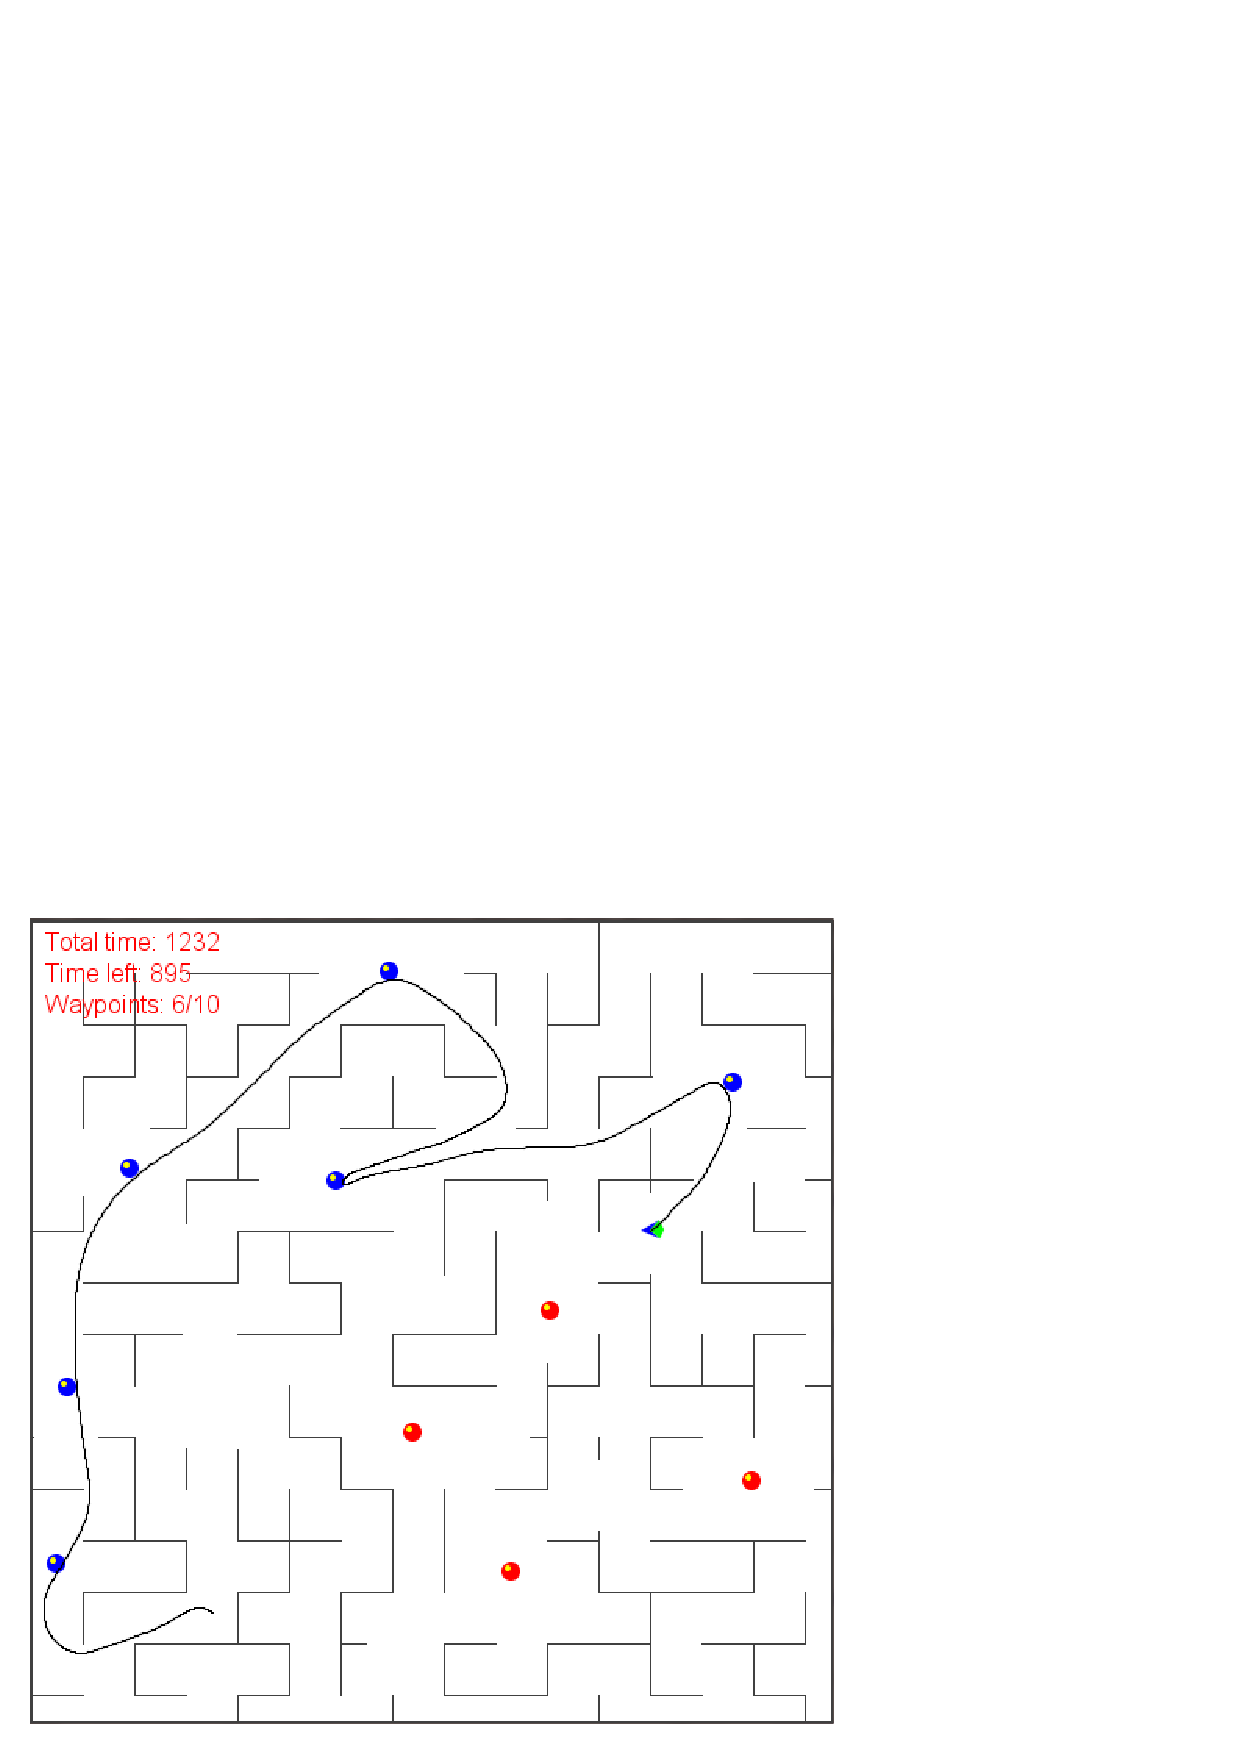
\includegraphics[scale=0.35]{img/ptspMap}
	\caption{Sample PTSP Map.}
	\label{fig:map}
	\end{center}
\end{figure}

The PTSP is a real-time game. For every cycle, the ship must supply an action to execute in no more than $40ms$. Additionally, there is a maximum time, depending on the number of waypoints in the map, that cannot be overspent when visiting the next waypoint. There are six different actions that can be provided to steer the ship. These actions are discrete and are divided into two different inputs: acceleration (which can be \textit{on} or \textit{off}) and steering (which can be \textit{left}, \textit{right} or \textit{straight}). The action applied modifies the position, velocity and orientation of the ship. 

The PTSP featured in two competitions in 2012 which took place at international IEEE conferences: the World Congress On Computational Intelligence (WCCI) and the Conference on Computational Intelligence and Games (CIG). The interested reader can found more information about the competition (game, rules and framework), as well as background for TSP solvers, navigation algorithms and similar real-time game competitions at~\cite{Perez2012}. The winner of both competitions was a Monte Carlo Tree Search approach based on macro-actions and a physics-based TSP route planner~\cite{Powley2012}. 

\section{Solving the PTSP} \label{sec:solve}

An obvious way to tackle the PTSP is by approaching the two sub-problems it constitutes: the order of waypoints to follow and the procedure to drive the ship to each of them. In other words, it is necessary to tackle both short-term and long-term planning tasks, whilst taking into account the interdependencies between the two (i.e. the physics of the game).

The focus of this paper is on the driving procedure. The order of waypoints followed is the same for the different algorithms presented in this study. This route is calculated at the beginning of the game, during initialization, and it remains available to the controller for the whole game. The calculated route takes the physics of the game into account: each given route has an associated cost assigned by a procedure that decomposes the route into straight-line obstacle free segments. The time taken to complete each one of these segments is estimated using the physics of the game and keeping the speed at the end of the segments. A penalization factor is applied at the end of each segment, related to the angle between the current and next segment in the route. This factor reduces the speed of the agent after each segment, in order to approximate the effects of turns in the trajectory of the ship. It has been determined~\cite{Perez2012a} that those routes involving fewer changes of direction, even when the distance travelled is higher, usually provide better results.


\subsection{Single versus Macro Actions} \label{sec:macro}

As stated in Section~\ref{sec:ptsp}, there are six different actions that can be applied at each time step. Each action must be decided within the 40ms of time allowed for the controller to choose a move. A good quality solution for a PTSP map with $10$ waypoints requires between $1000$ (in the maps with less obstacles) and $2000$ (in more complex ones, as in the one shown in Figure~\ref{fig:map}) time steps or action decisions. This creates a search space of $(1000,2000) \rightarrow (6^{1000}, 6^{2000})$, which obviously makes it impossible to calculate the optimal route within the time limitations given. 

A reasonable reduction of this search space can be achieved by limiting how far ahead in the game the algorithms can look. As described before, the order of waypoints is calculated during the initialization process. The controller has information about how many and which waypoints have been already visited, and it knows which ones are the next $N$ waypoints to be collected. If only the next $2$ waypoints are accounted, and according to the game length estimates, the search space size is reduced to $(6^{2 \times 100}, 6^{2 \times 200})$ (assuming that the ship usually takes $100$ to $200$ actions per waypoint).

More reduction can be achieved by introducing the concept of \textit{macro-actions}. In this paper a macro-action is just the repetition of the same action for $L$ consecutive time steps. The impact of changing a single action in a given trajectory is not necessarily big, so high quality solutions may still be found by not using such fine-grained precision. For instance, choosing a macro-action \textit{length} (defined as the number of repetitions per macro-action) of $10$, reduces the search space size to $(6^{20}, 6^{40})$. Different values of $L$ are used during the experiments described in this paper in order to show how this parameter affects the performance of each one of the algorithms described.

Macro-actions have a second and important advantage: they allow longer evaluations to execute before taking a decision (through several game steps). In a single action scenario, each algorithm has only 40ms to decide the next action to execute. However, in the case of a macro-action that is composed by $L$ single actions, each macro-action has $L \times 40$ms to decide the move, as the previous macro-action needs $L$ time steps to be completed (with the exception of the very first move, where there is no previous action). Algorithm~\ref{alg:macro} defines a handler for macro-actions. 

\begin{algorithm}[!ht]
\begin{algorithmic}[1]
\Function{GetAction}{$GameState:gs$}
	\If{$\Call{IsGameFirstAction}{gs}$}
		\State $actionToRun \gets \Call{DecideMacroAction}{gs}$ \label{lst:line:firstTime}
	\Else
		\For{$i = 0 \to remainingActions$} 
			\State $\Call{gs.Advance}{actionToRun}$  \label{lst:line:advance}
		\EndFor 
		\If{$remainingActions > 0$}		
			\If{$resetAlgorithm$}
				\State $\Call{Algorithm.Reset}{gs}$
				\State $resetAlgorithm \gets false$	
			\EndIf
			\State $\Call{Algorithm.NextMove}{gs}$ \label{lst:line:eval}
		\Else \Comment{$remainingActions$ is $0$}
			\State $actionToRun \gets \Call{DecideMacroAction}{gs}$ \label{lst:line:backTo0}
		\EndIf
	\EndIf
	\State $remainingActions = (remainingActions - 1)$
	\State \Return $actionToRun$
\EndFunction

\State
\Function{DecideMacroAction}{$GameState:gs$} \label{lst:line:decideMacroStart}
	\State $actionToRun \gets \Call{Algorithm.NextMove}{gs}$
	\State $remainingActions \gets L$
	\State $resetAlgorithm \gets true$	
	\State \Return $actionToRun$ \label{lst:line:decideMacroEnd}
\EndFunction
\end{algorithmic}
\caption{Algorithm to handle macro-actions.}
\label{alg:macro}
\end{algorithm}

The algorithm works as follows: the function $GetAction$, called every game step, must return a (single) action to execute in the current step. When the function is called for the first time (line~\ref{lst:line:firstTime}), or the number of remaining actions is back to $0$ (line~\ref{lst:line:backTo0}), the function $DecideMacroAction$ is called. This function (lines~\ref{lst:line:decideMacroStart} to~\ref{lst:line:decideMacroEnd}) executes the decision algorithm (which could be tree search, evolution or random search), that is in charge of returning the move to make, and sets a counter ($remainingActions$) to the length of the macro-action ($L$). Before returning the action to run, it indicates that the next cycle in the algorithm needs to be reset.

In cases where the current step is not the first action of the game, the state is advanced until the end of the macro-action that is currently being executed (line~\ref{lst:line:advance}). This way, the decision algorithm can start the simulation from the moment in time when the current macro-action will have finished. The algorithm is then reset (if it was previously indicated to do so by $DecideMacroAction$) and finally evaluates the current state to take the next move (line~\ref{lst:line:eval}). 

Note that in this case the value returned by $NextMove$ is ignored: the action to be executed is $actionToRun$, decided in a different time step. The objective of this call is to keep building on the knowledge the algorithm is gathering in order to decide the next macro-action (which effectively happens in $DecideMacroAction$) while the ship makes the move from the \texttt{previous} macro-action decision. Therefore, $Algorithm.NextMove$ is called $L$ times, but only in the last one is a real decision made. 

It is important to note that the algorithms determine a best solution of $N$ macro-actions with $L$ single actions per macro-action. However, only the \texttt{first} macro-action of the best solution is finally handled and executed by the controller. Once the best individual has been determined after $L$ iterations, the first macro-action is used and the rest are discarded, as the algorithm is reset at that point. The decision algorithm is in charge of keeping its internal state from one call to the next, replying within the allowed time budget and resetting itself when $Algorithm.Reset$ is called.

\subsection{Score function} \label{sec:score}

Even the usage of macro-actions does not ensure that any succession of $N$ actions reaches the next two waypoints in the (pre-planned) route: it is unlikely that a random sequence of actions visits even one of them. In fact, the vast majority of random trajectories will not visit any waypoints at all. It is thus necessary to improve the granularity of the rewards by defining a function that is able to distinguish the quality of the different trajectories, by scoring the game in a given state. This function is defined independently from the algorithm that is going to use it, so the research is centred on how the search space is explored by the different algorithms.

The score function takes into account the following parameters: distance and state (visited/unvisited) of the next two waypoints in the route, time spent since the beginning of the game and collisions in the current step. The final score is the addition of four different values. The first one is given by the \textit{distance points}, which is defined as follows: being $d_w$ the distance to the waypoint $w$, the reward for distance $r_{dw}$ is set to $10000-d_w$. If the first waypoint is not visited, it is set to $r_{d1}$.  However, if the first waypoint is visited, this is set to $r_{d1}$ plus a reward value ($10000$). The other values for the score function are given by the waypoints visited (number of visited waypoints, out of the next two, multiplied by a reward factor, $1000$), time spent (set to $10000$ minus the time spent during the game) and collisions ($-100$ if a collision is happening in this step).

%Figure~\ref{fig:scheme} shows a scheme of the controllers employed in this study. All four controllers described in upcoming sections share this same framework.
%
%\begin{figure} [!b]
%	\begin{center}
%	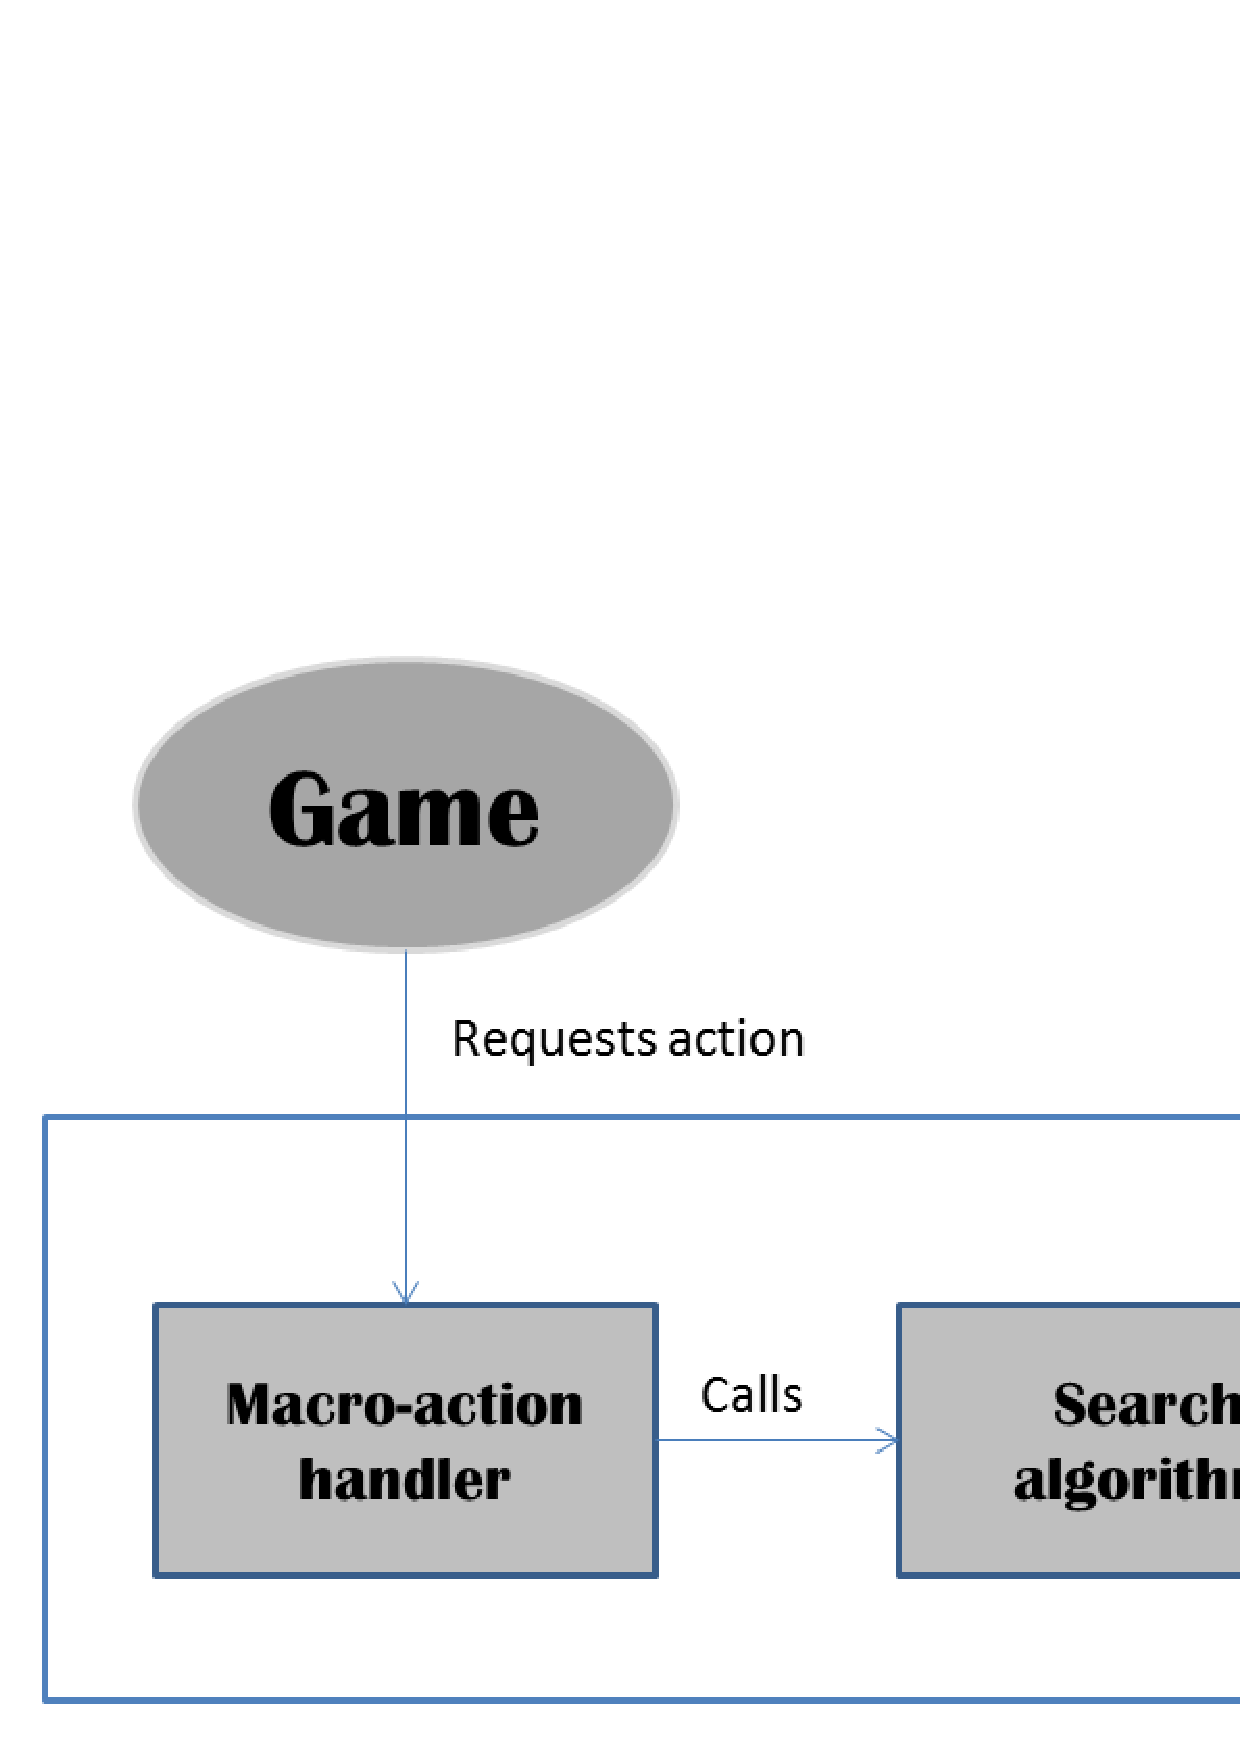
\includegraphics[scale=0.25]{img/schemeB}
%	\caption{General controller framework.}
%	\label{fig:scheme}
%	\end{center}
%\end{figure}

\subsection{Genetic Algorithm}

The two versions of the Genetic Algorithm (GA) employed in this study are simple evolutionary algorithms, where each individual encodes a group of macro-actions using integers. Each one of the possible six actions is represented with a number from $0$ to $5$. Note that each one of these genes represents a macro-action: the action denoted by the gene is repeated for $L$ steps in the game where $L$ is defined in the experimental setup. 

All individuals in the population have a fixed length, as defined in the experimental setup phase. As the algorithm is meant to run online (i.e. while the game is actually being played), a small population size of $10$ individuals is used in order to be able to evolve over a large number of generations. Elitism is used to automatically promote the best $2$ individuals of each generation to the next. Evolution is stopped when $(40ms - \epsilon)$ is reached. $\epsilon$ is introduced in order not to use more time than allowed to provide an action.

Individuals are initialized uniformly at random such that each gene can take any value between $0$ and $5$. This initialization happens many times during each game: in the first step of the game and every $L$ moves, as described in Section~\ref{sec:macro}. Mutation is used with different rates: $0.2$, $0.5$ and $0.8$. Each time a gene is mutated, only one of the two inputs involved in the action is randomly chosen to be changed. If acceleration is changed, the value is flipped from \textit{On} to \textit{Off}, or vice versa. If steering is modified, \textit{left} and \textit{right} mutate to \textit{straight}, while \textit{straight} can mutate to \textit{right} or \textit{left} at $50\%$ chance. This procedure was designed in order to transit smoothly between actions. Tournaments of size $3$ are used to select individuals for uniform crossover.

Finally, the evaluation of an individual is performed by the following mechanism: given an individual with $N$ macro-actions and $L$ single actions per macro-action, the game is advanced, using the forward model mentioned in Section~\ref{sec:ptsp}, applying the $N \times L$ actions defined in the individual. Then, the resultant game state is evaluated with the score function defined in Section~\ref{sec:score}.

Two different variants are employed in this study. The first one (referred to as GAC), implements all features described above. The second one (herein simply referred to as GA) does not employ tournament selection nor crossover. 


\subsection{Monte Carlo Tree Search} \label{sec:uct}

MCTS is a simulation-based algorithm that builds a tree in memory. Each node keeps track of statistics relating to how often a move is played from a state ($N(s,a)$), how many times each move is played from a state ($N(s)$) and the value of the average reward ($Q(s,a)$). The algorithm presented here uses the Upper Confidence Bound (UCB1; see Equation~\ref{eq:ucb1}) equation at each decision node to balance between exploration and exploitation. This balance is achieved by setting the value of $C$, which provides the algorithm with more or less exploration, at the expense of exploitation. A commonly used value is $\sqrt{2}$, as it balances both facets of the search when the rewards are normalized between $0$ and $1$.

\begin{equation}	\label{eq:ucb1}
a^* = \argmax_{a \in A(s)} \left\{Q(s,a) + C \sqrt{\frac{ \ln N(s) }{ N(s,a) }}\right\}
\end{equation}
 

The MCTS algorithm is executed in several steps~\cite{Gelly2006a}: at the very beginning of the algorithm, the tree is composed of only the root node, which is a representation of the current state of the game. During the \textit{selection} step, the tree is navigated from the root until a maximum depth has been reached. If a node has as many children as the available number of actions from that position, UCB1 is used as tree policy. Otherwise, a new node is added as a child of the current one (\textit{expansion} phase) and the \textit{simulation} phase starts. At this point, MCTS executes a Monte Carlo simulation (or roll-out; default policy) from the expanded node until the pre-defined depth, where the state of the game is evaluated. Finally, during the \textit{back-propagation} step, the statistics $N(s)$, $N(s,a)$ and $Q(s,a)$ are updated for each node traversed, using the reward obtained in the evaluation of the state. These steps are executed in a loop until a termination criteria is met (in the case presented here, when the time budget is consumed). Figure~\ref{fig:mcts} summarizes the steps of the algorithm.

\begin{figure} [!t]
	\begin{center}
	\includegraphics[scale=0.25,natwidth=708,natheight=484]{img/mcts.png}
	\caption{MCTS algorithm steps.}
	\label{fig:mcts}
	\end{center}
\end{figure}

In the problem presented in this paper, each of the actions in the tree is a macro-action. This means that, when navigating through the tree, $L$ single actions must be performed to move from one state to the next, defined by the action picked. In most games, the depth of the tree is limited by the number of moves required to reach an end game state. In the case of the PTSP, the end of the game is usually not reached, so the maximum depth is determined by the number and length of the macro-actions, defined differently for each experiment, bringing it closer to rolling horizon search then normal MCTS. 

The tree is preserved from one game step to the next (i.e. during $L$ moves) and is discarded every time the algorithm is reset. When the controller asks for a move, the action chosen is the one that corresponds to the child of the root with the maximum expected value $Q(s,a)$.



\subsection{Random Search}

Random Search (RS) is a simple algorithm that creates random solutions of a specified length. During the allocated time, new individuals are created uniformly at random and evaluated, keeping the best solution found so far. As in the other solvers, the best solution is forgotten every time the algorithm is told to be reset. The motivation behind including RS in this research is the good results obtained by the GA with high mutation rates. Thus, it is important to investigate how the results given by RS compare to those.

\section{Experimentation} \label{sec:exp}

\subsection{Experimental Setup} \label{sec:setup}

The experiments presented in this paper have been carried out on 10 different maps, running 20 matches per maze. Hence, each configuration has been executed during $200$ games, in order to get reliable results.\footnote{All experiments were performed in a dedicated server Intel Core i5 machine, 2.90GHz 6MB, and 4GB of memory.} The maps are those distributed within the framework of the PTSP competition.\footnote{\url{www.ptsp-game.net}} 

Five different configurations are used for each algorithm, varying the number of macro-actions ($N$) and the number of single actions per macro-action ($L$). These configurations, indicated by the pairs ($N$,$L$), are as follows: \[\{(50,1),(24,5),(12,10),(8,15),(6,20)\}\] The last four configurations share the property of foreseeing the same distance into the future: $N \times L = 120$. The only exception is the first configuration, where $L=1$, this is considered as a special case as no macro-actions are used.

A key aspect for interpreting the results is to understand how games are evaluated. If two single games are to be compared, following the rules of PTSP, it is simple to determine which game is better: the solution that visits more waypoints is the best. If both solutions visit the same number of waypoints, the one that does so in the minimum number of time steps wins.

However, when several matches are played in the same map, determining the winner is not that simple. One initial approach is to calculate the averages of waypoints visited and time spent, following the same criteria used in the single game scenario. The problem with this approach is that the difference between two solutions, taken as the average of waypoints visited, can be quite small (less than one waypoint), while the difference in time steps can be large. For instance, imagine a scenario where two solvers ($A$ and $B$) obtain an average of waypoints ($w_i$) of $w_a=9.51$ and $w_b=9.47$, and an average of time steps ($t_i$) of $t_a=1650$ and $t_b=1100$. The traditional comparison would say that $A$ wins (because $w_a>w_b$), but actually $B$ is much faster than $A$ ($t_b \ll t_a$) with a very small waypoint difference. Intuitively, $B$ seems to be doing a better job.

A possible solution to this problem is to calculate the ratio $r_i = t_i / w_i$ that approximates the time taken to visit a single waypoint. The drawback to this approach is that it does not provide a reliable comparison when one of the solvers visits a small number of waypoints (or even $0$). Therefore, the following two features have been analysed:
\begin{itemize}
\item \textit{Efficacy}: number of waypoints visited, on average. The higher this value, the better the solution provided.
\item \textit{Efficiency}: ratio $r_i = t_i / w_i$, but only for those matches where $w_i$ equals the number of waypoints of the map. The goal is to minimize this value, as it represents faster drivers.
\end{itemize}

\subsection{Results and analysis} \label{sec:wcci}

\subsubsection{40 milliseconds} 

Table~\ref{tab:visits40} shows the number of waypoints visited on average, including the standard error. The first notable aspect is that, out of the algorithms presented here, when no macro-actions are provided ($L=1$), only MCTS is able to solve the problem up to a point. The other three algorithms cannot complete the game, not getting more than one waypoint in some rare cases. When the length of macro-action is increased to $5$, on average all algorithms achieve close to all waypoints. Excellent efficacy is obtained where the macro-action length is raised to $15$, which seems to be the overall best value for this parameter. In general, the GA (especially with high mutation rates) seems to be the algorithm that obtains the best efficacy.

\begin{table*}[!ht]
\begin{center}
\begin{tabular}{|>{\centering\arraybackslash}m{0.3cm}|>{\centering\arraybackslash}m{1.45cm}|>{\centering\arraybackslash}m{1.45cm}|>{\centering\arraybackslash}m{1.45cm}|>{\centering\arraybackslash}m{1.45cm}|>{\centering\arraybackslash}m{1.75cm}|>{\centering\arraybackslash}m{1.75cm}|>{\centering\arraybackslash}m{1.9cm}|>{\centering\arraybackslash}m{1.75cm}|}
\hline
 & \multicolumn{8}{c|}{Average Waypoints Visited} \\ 
\hline
$L$ & MCTS & RS & GA 0.2 & GA 0.5 & GA 0.8 & GAC 0.2 & GAC 0.5 & GAC 0.8\\ 
\hline
1 & $7.66 \pm 0.25$ & $0.03 \pm 0.01$ & $0.03 \pm 0.01$ & $0.05 \pm 0.01$ & $0.01 \pm 0.01$ & $0.03 \pm 0.01$ & $0.02 \pm 0.01$ & $0.01 \pm 0.01$\\
\hline
5 & $9.62 \pm 0.11$ & $9.76 \pm 0.08$ & $9.87 \pm 0.06$ & $9.89 \pm 0.06$ & $9.86 \pm 0.06$ & $9.91 \pm 0.05$ & $9.9 \pm 0.05$ & $9.69 \pm 0.09$ \\
\hline
10 & $9.62 \pm 0.12$ & $9.95 \pm 0.03$ & $9.96 \pm 0.03$ & $10.0 \pm 0.0$ & $10.0 \pm 0.0$ & $9.96 \pm 0.04$ & $9.91 \pm 0.06$ & $9.96 \pm 0.03$ \\ 
\hline
15 & $10.0 \pm 0.0$ & $10.0 \pm 0.0$ & $10.0 \pm 0.0$ & $10.0 \pm 0.0$ & $10.0 \pm 0.0$ & $10.0 \pm 0.0$ & $10.0 \pm 0.0$ & $10.0 \pm 0.0$ \\
\hline
20 & $9.97 \pm 0.03$ & $9.95 \pm 0.04$ & $10.0 \pm 0.0$ & $10.0 \pm 0.0$ & $10.0 \pm 0.0$ & $9.97 \pm 0.02$ & $9.98 \pm 0.02$ & $9.92 \pm 0.04$ \\
\hline
\end{tabular}
\caption{Waypoint visits with $40$ms per time step.}
\label{tab:visits40}
\end{center}
\end{table*}


Regarding efficiency, Figure~\ref{fig:ratDetGA} shows the ratio average with standard error obtained with the GA (very similar results are obtained with GAC). One of the first things to note is that the mutation rate that obtains the best solutions is $0.5$, for both evolutionary algorithms, especially when the macro-action length is $10$ or lower. It is interesting to see how the distinct mutation rates make the algorithm behave differently: it is clear that a higher mutation rate works better with longer macro-actions, obtaining similar results to $0.5$. On the other hand, although rate $0.5$ is still the best, $0.2$ provides better results than $0.8$ for smaller values of $L$. This is confirmed by a Mann-Whitney-Wilcoxon statistical test (MW-test) run on this data: GA-$0.5$ is better than GA-$0.8$ for $L = 5$ and $10$ (p-values of $0.006$ and $0.041$, respectively), while GA-$0.5$ is faster than GA-$0.2$ for higher values of $L$ (p-values of $0.046$ and $0.022$ for $L = 15,20$).

\begin{figure} [!b]
	\begin{center}
	\includegraphics[width=0.75\columnwidth,natwidth=970,natheight=771]{img/GAmut40ms.png}
	\caption{Ratio (time/waypoints) results for GA.}
	\label{fig:ratDetGA}
	\end{center}
\end{figure}

Figure~\ref{fig:ratDetAll} shows the ratio average and standard error of RS, MCTS, GA and GAC (both with mutation rate $0.5$). One initial result to note is that the 2012 PTSP winner algorithm (MCTS) is no better than GA or GAC in any of the macro-action lengths tested (with the exception, as mentioned earlier, of $L=1$, which obtains a ratio of $168.37 \pm 7.7$). Actually, although overall there is no statistical difference, GA and GAC get better results than MCTS in some of the maps tested (see Section~\ref{sec:byMap}). It is also worthwhile mentioning that $L=15$ provides the best results for all algorithms. In fact, these results are compatible with previous studies: Powley et al.~\cite{Powley2012} used $L=15$ in their MCTS entry that won the 2012 WCCI competition. 

\begin{figure} [!b]
	\begin{center}
	\includegraphics[width=0.75\columnwidth,natwidth=1025,natheight=769]{img/Allmut40ms.png}
	\caption{Ratio (time/waypoints) results.}
	\label{fig:ratDetAll}
	\end{center}
\end{figure}

Finally, we observe an interesting phenomenon: while RS is clearly worse than the other algorithms in lower macro action-lengths ($L = 5,10$), the performance of all algorithms converges to the same performance when the maximum value of $L$ is reached. 

A possible explanation for this effect is as follows: for the maximum macro-action length ($L=20$), the length of the solution (or individual) that is being evaluated is $N=6$, providing $6^{6} \approx 3 \times 10^5$ combinations. This evaluation performs single actions during $L \times N = 120$ time steps, but remember that only the first macro-action is finally performed in the actual game, discarding the rest of the individual actions (as explained in Section~\ref{sec:macro}). Clearly, not all the actions in the sequence of $120$ moves are equally important; actions chosen at the beginning of this sequence produce a higher impact in the overall trajectory followed by the ship. Therefore, it is fair to assume that, for instance, the first half of the individual ($60$ actions) is more relevant for the search than the second. In the case of $L=20$, this is encoded in the first $3$ genes, which provides $6^{3} = 216$ different possibilities.  This is a very reduced search space where even random search can find a good solution (especially considering the amount of evaluations performed per cycle, as shown in Section~\ref{sec:eval}).

In the cases where $L=5$ or $L=10$, the same amount of look ahead ($60$ single actions) is obtained with $12$ and $6$ genes, which provides a search space of $6^{12} \approx 2 \times 10^9$, and $6^{6} \approx 3 \times 10^5$ respectively. In these more complex scenarios, the search space is better explored by both GAs (and MCTS) than by RS.

\subsubsection{80 milliseconds} \label{sec:eighty}

All the experiments described above were repeated with the decision time doubled to $80$ms. For the sake of space, these results are not detailed here, but they are consistent with the results obtained from spending $40$ms per cycle.

All the algorithms perform slightly better when more time is permitted, as would be expected. For instance, GA-$0.5$ obtains the best performance when $L=15$, with a ratio of $138.17 \pm 1.56$, about three units faster than the results achieved in $40$ms. Again, the relationship between the different algorithms is maintained: all algorithms perform better with $L=15$ and their performances get closer as the size of macro-action approaches $20$.




\subsection{Results by map} \label{sec:byMap}

These results can also be analysed on a map-by-map basis. Figure~\ref{fig:bars10} represents the ratio achieved by each algorithm in every map of this setup (remember lower is better). First of all, it is interesting to see how the overall performance of the algorithms changes depending on the map presented. For instance, map $9$ (the one depicted in Figure~\ref{fig:map}) happens to be especially complex. All algorithms obtain worse results in this map than, for instance, in map $10$, that contains no obstacles except the boundaries of the map. Regarding averages, GAC-$0.5$ obtains the best average of ratio per map in $7$ out of the $10$ different maps, whilst MCTS leads the rest.

\begin{figure} [!t]
	\begin{center}
	\includegraphics[width=0.75\columnwidth,natwidth=1021,natheight=765]{img/barsFinal10.png}
	\caption{Results per map, $L = 15$.}
	\label{fig:bars10}
	\end{center}
\end{figure}	

It is also possible to take the best results obtained in each map and compare them with the ones obtained in the WCCI PTSP competition. For instance, both GA and GAC obtain better solutions than the winner of the WCCI competition in $4$ out of the $10$ maps from the ones distributed with the competition framework. Similarly, MCTS outperforms the best results in two different maps.

The PTSP competition is quite strict regarding controllers that overspend the $40$ ms of time allowed per cycle, executing the action 0 (no acceleration, no steering) when this occurs. In the experiments presented in this paper, however, and for the sake of simplicity, this penalisation is ignored. In other words, controllers do use $40$ms, but should this time limit be violated (which may happen if a single evaluation takes more time than expected) the desired action is executed anyway. In order to verify if the results obtained are comparable with those from the competition, statistics relating to the number of times the controllers overspent the real-time limit were extracted. This phenomenon occurs in only between $0.1\%$ and $0.03\%$ of the total game cycles in a game, which suggests that, even if the results cannot be fairly considered as new records for those maps, the performance achieved by the algorithms presented in this paper is significant and is comparable to some extent.

\subsection{Number of evaluations} \label{sec:eval}

Another aspect worth mentioning is the number of evaluations (or calls to the score function) performed every game cycle.  MCTS is able to perform more evaluations per cycle, going from about $950$ when $L=5$ to $3000$ if $L=20$, while the other algorithms range between $330$ and $370$. The main reason for this being that MCTS stores intermediate states of the game in the tree, and is able to reuse this information during the simulations performed in a game cycle, whereas the other three algorithms execute all the actions encoded in each individual, from the first one to the last, producing a more expensive and hence slower evaluation.

The difference between both $GAs$ and $RS$ depends on the overhead of the algorithm (and not on the evaluation itself, which takes the same time for all of them): as shown in Figure~\ref{fig:evals}, $RS$ is the more efficient because of its simplicity, followed by $GA$ and then $GAC$, which is the slowest due to the cost of using selection and crossover. $MCTS$ is not included in this picture for the sake of clarity.

\begin{figure} [!t]
	\begin{center}
	\includegraphics[width=0.75\columnwidth,natwidth=1025,natheight=768]{img/evaluations.png}
	\caption{Evaluations per algorithm and $L$.}
	\label{fig:evals}
	\end{center}
\end{figure}

It is interesting to see how both GAs obtain equivalent (sometimes better) solutions than MCTS, the winner of the 2012 PTSP competition, even when they execute much fewer evaluations per game cycle.

\section{Conclusions} \label{sec:conc}

This paper compared the performance of several different search techniques for the PTSP, a real-time game where an action must be supplied every $40$ms. The PTSP resembles many modern games where the players need to move providing actions within a few milliseconds, which allows to extrapolate these conclusions to that type of games. The algorithms considered were random search (RS), two different evolutionary algorithms (GA and GAC) and Monte Carlo Tree Search (MCTS). For this, a rolling horizon version for the evolutionary algorithms is introduced. The search space is by using macro-actions, where each one simply repeats a low-level action a specified number of times, as has previously been shown to be successful~\cite{Powley2012}. The experiments were performed on the maps distributed with the PTSP competition enabling a direct comparison with the competition's results.

MCTS was the only algorithm able to produce relatively good solutions when no macro-actions were used. The fact that this algorithm stores information in the tree allows for a more efficient search when the search space is vast. However, the best results were obtained using macro-actions, more specifically where a macro-action length of $15$ was used. In this case, GAC and MCTS obtained better solutions on each one of the maps, in some cases achieving better results than those from the PTSP competition. The concept of macro actions is in no way restricted to the PTSP and may equally well be applied to the majority of real-time video games. Examples are high level commands in strategy games of first person shooters, where the use of macro-actions instead of low level orders enhances the performance of search algorithms due to a reduction of the search space.

Another important contribution of this paper is understanding how different discretizations of the search space affect the performance of the algorithms in this game. On the one hand, if the granularity is fine (small macro-action lengths, such as $L = 5, 10$), the search algorithm can benefit from artefacts such as the genetic operators. On the other hand, if the granularity is coarse the fitness landscape is rough, and the rolling horizon effect enables random search to perform as
well as the other algorithms. Finally, it is worth mentioning that both GAs obtained very good solutions while performing fewer evaluations than the other techniques. This would suggest that the search for solutions is more efficient in these two algorithms.  This is significant, suggesting that evolutionary algorithms offer an interesting alternative to MCTS for general video game agent controllers when applied in this on-line rolling horizon mode.

\section{Acknowledgments}
This work was supported by EPSRC grant EP/H048588/1. %Anonymous

\bibliographystyle{abbrv}
\bibliography{biblio}  
\end{document}